% Created 2024-03-19 Tue 12:48
% Intended LaTeX compiler: pdflatex
\documentclass[11pt,twocolumn]{article}
\usepackage[utf8]{inputenc}
\usepackage[T1]{fontenc}
\usepackage{graphicx}
\usepackage{longtable}
\usepackage{wrapfig}
\usepackage{rotating}
\usepackage[normalem]{ulem}
\usepackage{amsmath}
\usepackage{amssymb}
\usepackage{capt-of}
\usepackage{hyperref}
\hypersetup{colorlinks=true,linkcolor=blue,urlcolor=blue}
\usepackage{placeins}
\input article_setup.tex
\usepackage[nottoc,numbib]{tocbibind}
\renewcommand{\UrlFont}{\small\tt}
\renewcommand*{\UrlFont}{\footnotesize}
\hypersetup{colorlinks,citecolor=black,linkcolor=blue,urlcolor=magenta}
\usepackage{ragged2e}
\date{}
\title{}
\hypersetup{
 pdfauthor={Christopher Hepplewhite},
 pdftitle={},
 pdfkeywords={},
 pdfsubject={},
 pdfcreator={Emacs 28.1 (Org mode 9.5.2)}, 
 pdflang={English}}
\begin{document}

\author{L. Larrabee Strow, Sergio DeSouza-Machado, and Chris Hepplewhite}
\date{\today}
\title{\Large Year-1/Progress Report\\ \vspace{0.05in} \normalsize Award <>
  \\The Stand Alone Rapid Transmittance Algorithm - 2023-24.}
\maketitle

\section{Overview}
\label{sec:orgbcbb29e}
The stand alone radiative transfer algorithms (SARTA) include
parameterizations
of channel-averaged atmospheric layer transmittances. The original
wrapper code consists of a clear sky RTA, used in generating 
L2 retrieved products from level L1C Cloud Cleared Radiances
(CCRs), and a scattering version coupled to a novel representation
of clouds as two slabs (DeSouza-Machado et al 2018).
The 2-slab model takes advantage of the fact the
hyperspectral infrared radiances have very few degrees of freedom of cloud
information, allowing one to model the radiative transfer through two
equivalent layers instead of using multiple layers and phases in the
simulation. This is used at UMBC for single footprint
retrievals at the native sensor horizontal resolution.

The SARTA transmittances are derived from simulated
transmittances computed with UMBC's pseudo line-by-line algorithm kCARTA
(kCompressed Atmospheric Radiative Transfer Algorithm), which is the
reference forward model for SARTA. The line-by-line transmittances are
convolved to the instrument spectral line shapes (ILS) then fitted to a suite
of predictors used for the fast coefficients in SARTA.
The optical depths (ODs) used in kCARTA
primarily come from our custom in-house Matlab based line-by-line code
(UMBC-LBL). Additionally, kCARTA can be built with \cd and
\methane optical depths from the AER-LBLRTM code. Currently,
\methane line-mixing is not implemented in the UMBC-LBL so the AER-LBLRTM
option is used.
A complete description of both the underlying
line-by-line code (UMBC-LBL) and kCARTA can be found in
ref: DeSouza-Machado et al (2020).


\section{Year 1 Activities}
\label{sec:org49dfcce}

\subsection{Variables and gases included}
\label{sec:orgdf62763}

The following is a summary list of the processes, variables and gases
that are included in the SARTA.
Absorption by H2O, O3, CH4, CO, HNO3, N2O, SO2, NH3, HDO, CO2 including line mixing
and nonLTE,
surface thermal IR (TIR) emissivity and solar reflectivity, including atmospheric
path zenith angle
and solar zenith angle. The two-slab scattering version includes water droplet,
various ice and some dust habitats.

\subsection{Build Status at time of writing.}
\label{sec:org470fa20}

The current SARTA build uses the HITRAN 2020 updated line database.
The build status was reported in the last report, with the additional note
that all coefficient sets have been completed and verified during this
current reporting period.


\subsection{Testing, Validation and Tuning}
\label{sec:org3553705}

During this reporting period the SARTA has been used extensively and particularly
in bias analysis with global sensor observations, using
primarily the ECMWF atmospheric model fields with additional updated
greenhouse gas profiles (CO2, N2O, CH4) from ESRL. No additional tuning
has been identified as being necessary.


\subsection{Emissivity/Reflectivity Improvements}
\label{sec:org4cef460}

The updated sea surface emissivity models have been used in on-going bias analysis
with sensor observations and uncertainties are comparable to those from errors
due to water vapor continuum in the TIR window regions, being of the order 0.1 K.
Best regions for this study are over cloud-clear sub-tropical oceans with anticyclonic
conditions (descending hadley cell).

The challenges remain where they have always been; over mountains, ice-sheets, where
knowledge of both emisivity and skin temperature is poor.

In addition, the challenges of modelling short-wave reflectivity remain. The updated
Nalli (ref?) sea surface reflectivity models are available and initial studies indicate
a high degree of sensitivity to which model is chosen. Further study would be required
to demonstrate the best model to use. An alternative approach is to fit for the best
model of reflectivity from a large global data sample.

\subsubsection{Variation with View and Solar angle.}
\label{sec:orgb33ccf8}
In the thermal region (less than about 1900 cm-1) the effect of solar radiation is
ignored. At wavelengths shorter than this, when the solar zenith is less than 90-degrees
the solar radiation at the sensor is computed through the atmosphere to the surface
at the solar zenith angle and reflected from the surface to the sensor at the satellite
view angle. The total radiation includes the contribution from the atmospheric and
surface thermal emission at the satellite view angle. When the sum of the solar and
view angles is greater than about 84-degrees the optical depth receives an
extra multiplier for better approximation.

The question is how well constrained are the model errors at the larger view
and solar angles. Of particular interest is since the Aqua spacecraft began to drift
out of the A-train constellation how the effective slant paths through
the atmosphere might be changing. Drift in Equator crossing times is not of concern
here.
This can be evaluated by studying the obs:calc biases under these
conditions.

The mean daily solar zenith angle for a 3x5-deg lat/lon tile at the equator for all
FoVs for the whole mission is shown in Figure 1. Each point in this plot is for the
first day of each month during daylight.
It shows that early in the mission the orbit changed until
setling in 2007, then late 2021 began to drift.

\begin{figure}[htbp]
\centering
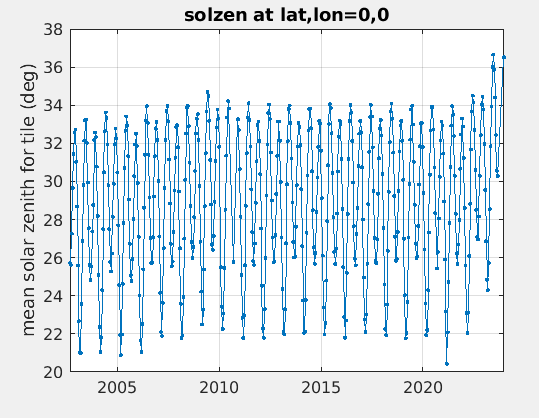
\includegraphics[width=\linewidth]{./Figs/SolZenVar_2002-2023.png}
\caption{\label{fig:org25b1817}Variation of Mean Solar Zenith angle near the equator.}
\end{figure}

The variation of the peak (or maximum) solar zenith angle varies around the globe
as a direct result of the polar sun-synchronous orbit and with time of year.
Since we are concerned with modelling the solar flux only daytime observations
are of interest. Figure 2 shows the maximum daytime solar zenith in a collection of
16-days in January 2023, the effect of polar day and night are obvious.

\begin{figure}[htbp]
\centering
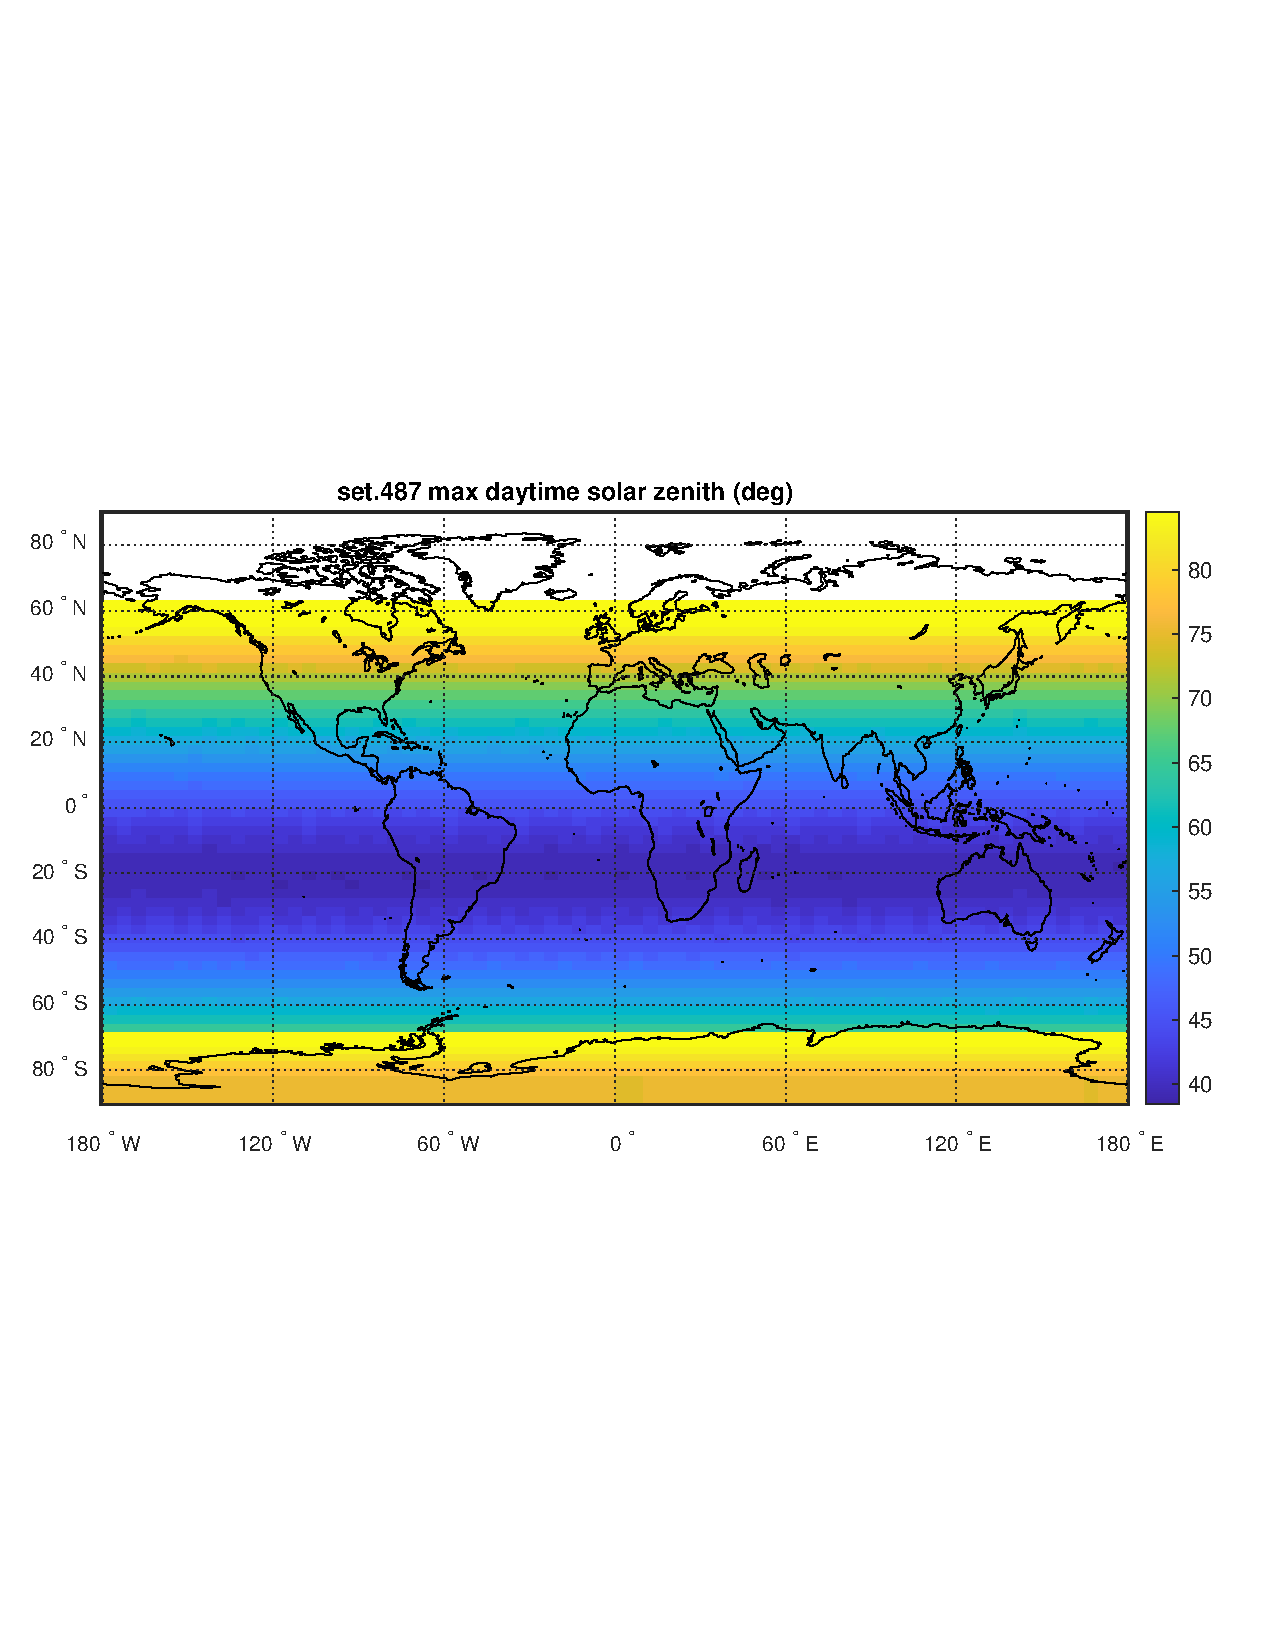
\includegraphics[width=\linewidth]{./Figs/set487_max_day_solzen_global_map.pdf}
\caption{\label{fig:orgb0aa297}Maximum solar zenith from 16-day collection Jan 2023.}
\end{figure}

Figure 3 shows the variation of the maximum daytime solar zenith for the mission
over two 3x5-deg lat/lon tiles over the mission. seleting a region near to the pole
would show increasing population of near 90-deg solr zenith as expected.

\begin{figure}[htbp]
\centering
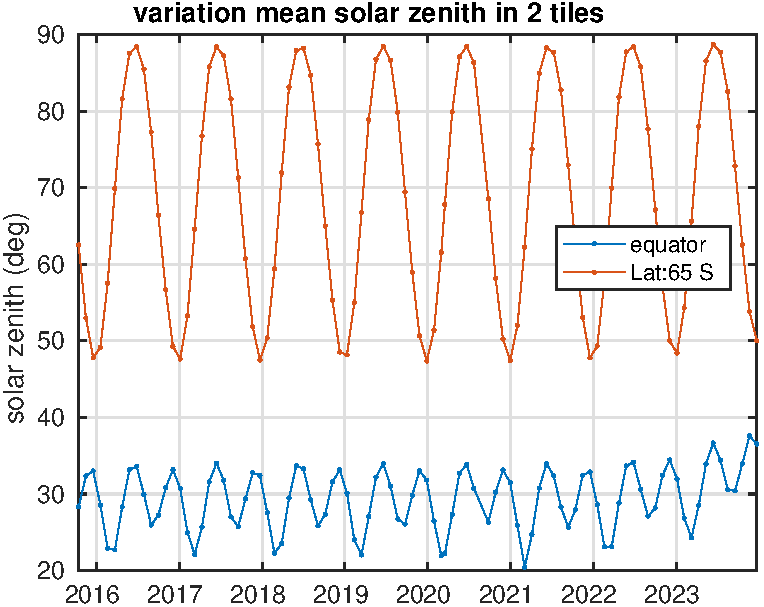
\includegraphics[width=\linewidth]{./Figs/solzen_mean_var_vs_time_two_tiles.pdf}
\caption{\label{fig:orgf6961e4}Variation of max. daytie solar zenith at two locations.}
\end{figure}

From this it is clear that solar zenith changes impact the tropical regions
more than at higher latitudes. Furthermore, the maximum solar zenith to-date have been
no more than 6-degrees at most peaking from 32 to 38-deg. High latitudes continue to
recieve daytime solar radiation all the way to 90-deg but more frequently.

The Satellite zenith view angles have, to first-order, not changed with the orbit drift.
There is a second-order change due to orbit altitude that is negligible for this
modelling work.

The accuracy of the SARTA top-of-atmosphere (TOA) radiance (Brightness Temperature)
can be determined by computing the bias of the observations and calculations for
large samples of data and how these vary with view and solar angles.

Figure 4 shows the bias as a function of satellite zenith for night-time observations
averaged for 16-days global ocean clear views for the complete spectral band.
Ignore the bandgap from 1650 to 2150 cm-1. This shows that the bias varies across the
satellite view angle range peaking between +/- 0.2 K in general, with overall mean
(not shown) close to zero Kelvin). The maximum view angle is about 58-degrees. This
result demonstrates that there is no sudden loss of accuracy at the extremens of
view angle for thermal flux.

\begin{figure}[htbp]
\centering
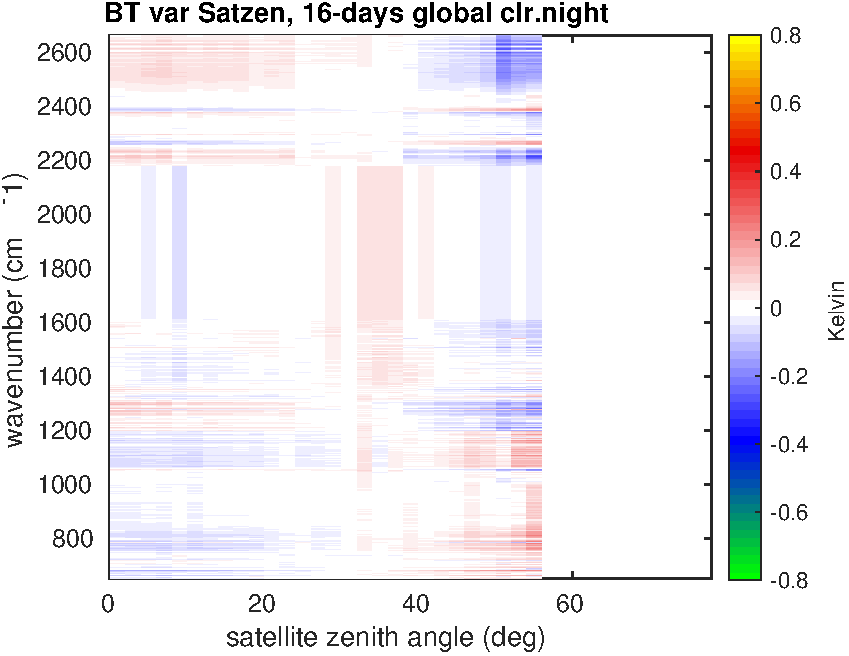
\includegraphics[width=\linewidth]{./Figs/airs_oc_bias_vs_satzen_wvn_16dy_gblclr_nite_pcolor.pdf}
\caption{\label{fig:org5337b0a}Variation of obs:calc bias global ocean clear night-time average 16-day period.}
\end{figure}

Figure 5 shows the same result as Fig.4 but for day-time observations. Ignore the band-gap
between 1650 to 2150 cm-1. Notice the large bias variation for the short-wave window region
due almost entirely to inaccurate model of sea surface reflectivity, which averages
close to zero (not shown).Also notice the variation in the CO2 band, due mainly to the
limitations of the non-LTE model (more on this in the next section), again which
averages close to zero (not shown). This result shows there is no sudden loss of
acuracy at the extreme view angles.

\begin{figure}[htbp]
\centering
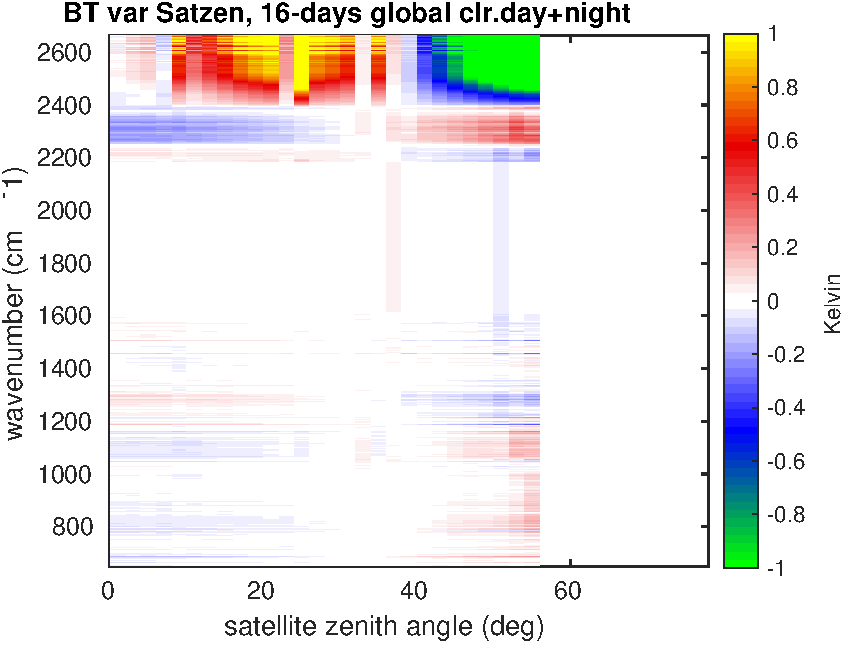
\includegraphics[width=\linewidth]{./Figs/airs_oc_bias_vs_satzen_wvn_16dy_gblclr_pcolor.pdf}
\caption{\label{fig:orgc152cf5}Variation of obs:calc bias global ocean clear day-time average 16-day period.}
\end{figure}

Figure 6 shows the same result as Fig.5 but as a function of all solar zenith angle
for all satellite view angles for global ocean clear views (day and night). Ignore
the band-gap 1650 to 2150 cm-1. It shows the same characteristics as Fig.5,
with the bias extended through the night. As before it shows there is no sudden
loss of accuracy.

\begin{figure}[htbp]
\centering
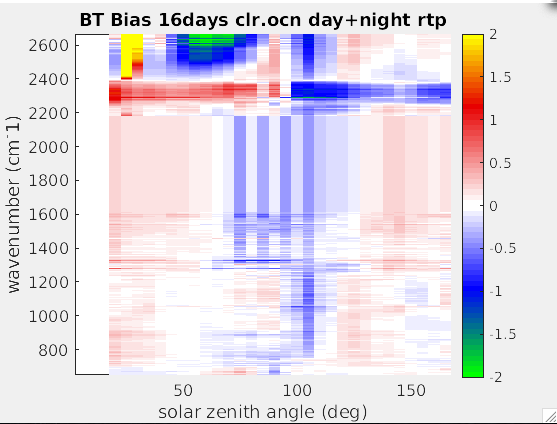
\includegraphics[width=\linewidth]{./Figs/airs_oc_bias_vs_solzen_day_night_glob_ocn_clr.png}
\caption{\label{fig:orgcb99237}Variation of obs:calc bias global ocean clear day and night average 16-day period.}
\end{figure}

The overall conclusion is that the effect of the orbit drift will shift the bias
characteristic slightly across the range of angles, but the effect is comparable
to overall uncertainties in the model.

\section{Non-LTE Emission}
\label{sec:org09593b6}

Since the last reporting period several different sets of predictors have been tried
for the regression to find new fast coefficients and these have so far not
found to perform better than the original set. One of the main limitations is
due to the null point of secant at 90-degrees. Since the new model extends to
nonLTE effect through to solar zenith 120-degrees. Previously the nonLTE was
tied to 89 degrees with zero nonLTE >= 90-degrees solar zenith.

A typical example of the model performance for a day of global randomly
sampled observations and calcs is shown in figure 7. This result includes
absorption and reflection beyond the CO2 band. The new model is version v2
and the original version v1. In each test run the local thermodynamic equilibrium (LTE)
results are the same (blue curves). The nonLTE results are different with the
v1 being perhaps slightly better.

\begin{figure}[htbp]
\centering
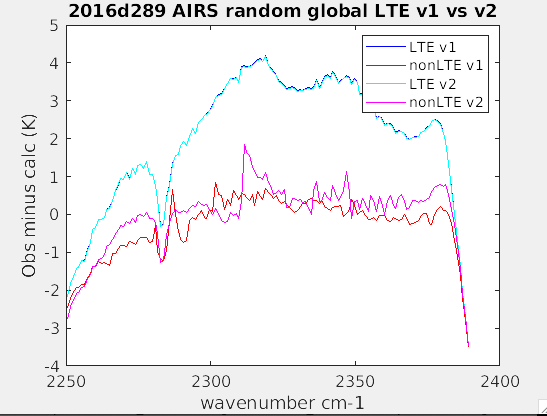
\includegraphics[width=\linewidth]{./Figs/airs_oc_bias_random_day_nlte.png}
\caption{\label{fig:org7e04f96}Old vs Extended nonLTE model.}
\end{figure}

At the time of writing a new approach is being evaluated in which a neural net
is to be trained on the 49 atmospheric profiles at 6 view and 19 solar angles
(and is being extended to the SAF set which is much larger). 


\section{References:}
\label{sec:org63b33b2}
DeSouza\_Machado et al. Atmos. Meas. Tech., 11, 529–550, 2018
\url{https://doi.org/10.5194/amt-11-529-2018}

DeSouza-Machado et al. Atmos. Meas. Tech., 13, 323–339, 2020
\url{https://doi.org/10.5194/amt-13-323-2020}
\end{document}